\documentclass{beamer}

\usepackage[utf8]{inputenc}
\usepackage[T1]{fontenc}
\usepackage{default}

\title{Music generation}
\author{T. Ardoin -- M. Dufraiss -- N. Lichtle -- A. Riou -- R. San Roman}
\date{25 Janvier 2019}

\begin{document}
\begin{frame}
	\maketitle
\end{frame}

\begin{frame}{Objectifs}
	Générer de la musique.
	\begin{description}
		\item[Dataset:] Un ensemble de partition sous forme de fichiers MIDI.
		\item[Sortie] Un fichier MIDI.
	\end{description}
\end{frame}

\section{Using GANs}
\begin{frame}{Midinet}
\begin{itemize}
	\item \textit{MidiNet: A Convolutional Generative Adversarial Network for Symbolic-domain Music Generation}
	
	by Li-Chia Yang, Szu-Yu Chou, Yi-Hsuan Yang in 2017.
	\item Uses CNN for the generator instead of RNN;
	\item Can be used to follow a melody or produce multitrack melody.
\end{itemize}
	
\end{frame}

\begin{frame}{Architecture}
\begin{figure}[h]
\centering
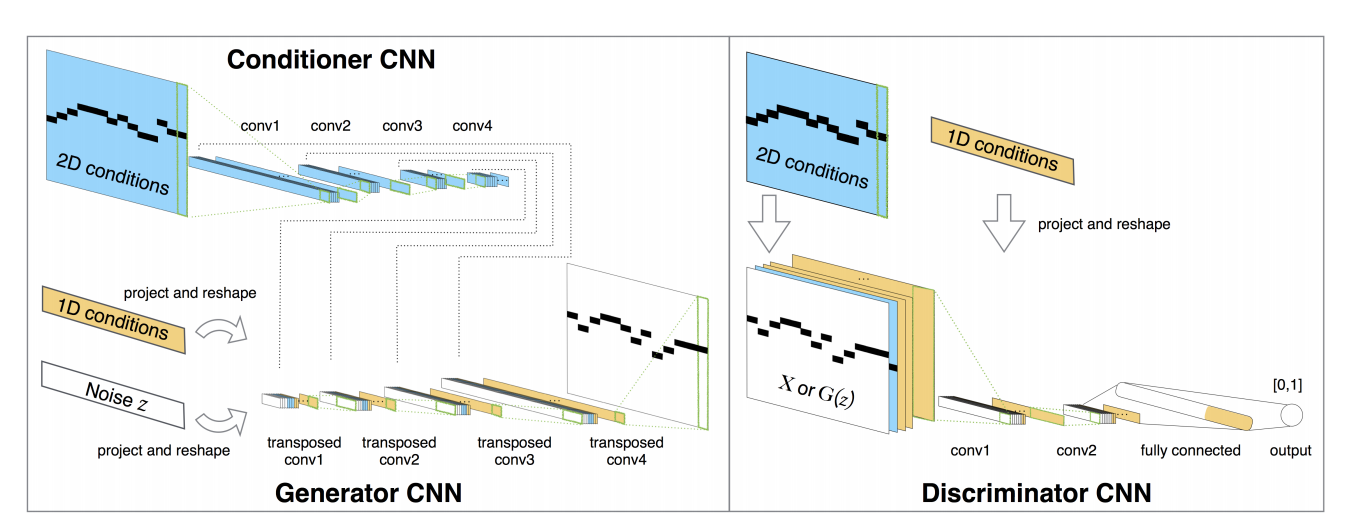
\includegraphics[width=1\linewidth]{midinet}
\caption{The architecture of the MidiNet Network}
\end{figure}
\end{frame}

\begin{frame}{Results}
\begin{itemize}
	\item The conditioner helps prevent mode collapse.
\end{itemize}
\begin{figure}[h]
\centering
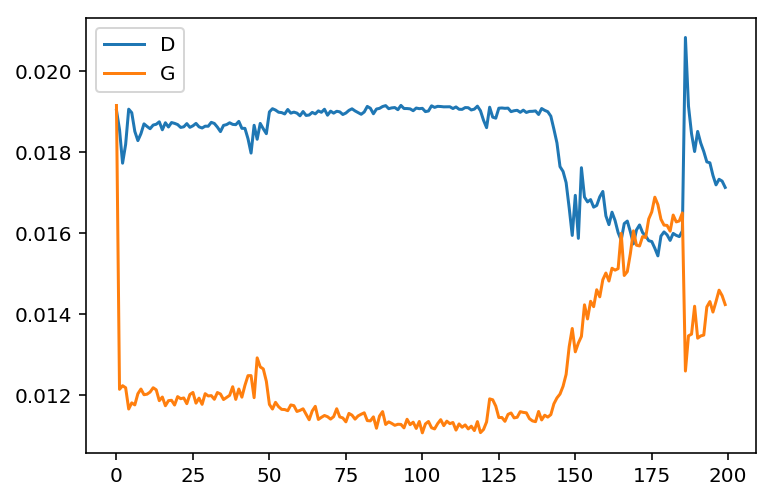
\includegraphics[width=0.6\linewidth]{loss_midinet_w_cond}
\end{figure}
\end{frame}

\section{Using VAEs}
\begin{frame}{MusicVAE}
\textit{A Hierarchical Latent Vector Model for Learning Long-Term Structure in Music}
by Adam Roberts, Jesse Engel, Colin Raffel, Curtis Hawthorne, Douglas Eck
\begin{itemize}
	\item Based on a variational autoencoder.
	\item Uses a hierarchical structure to have some long-term consistency.
\end{itemize}
\end{frame}

\begin{frame}{Architecture}
\begin{figure}[h]
\centering
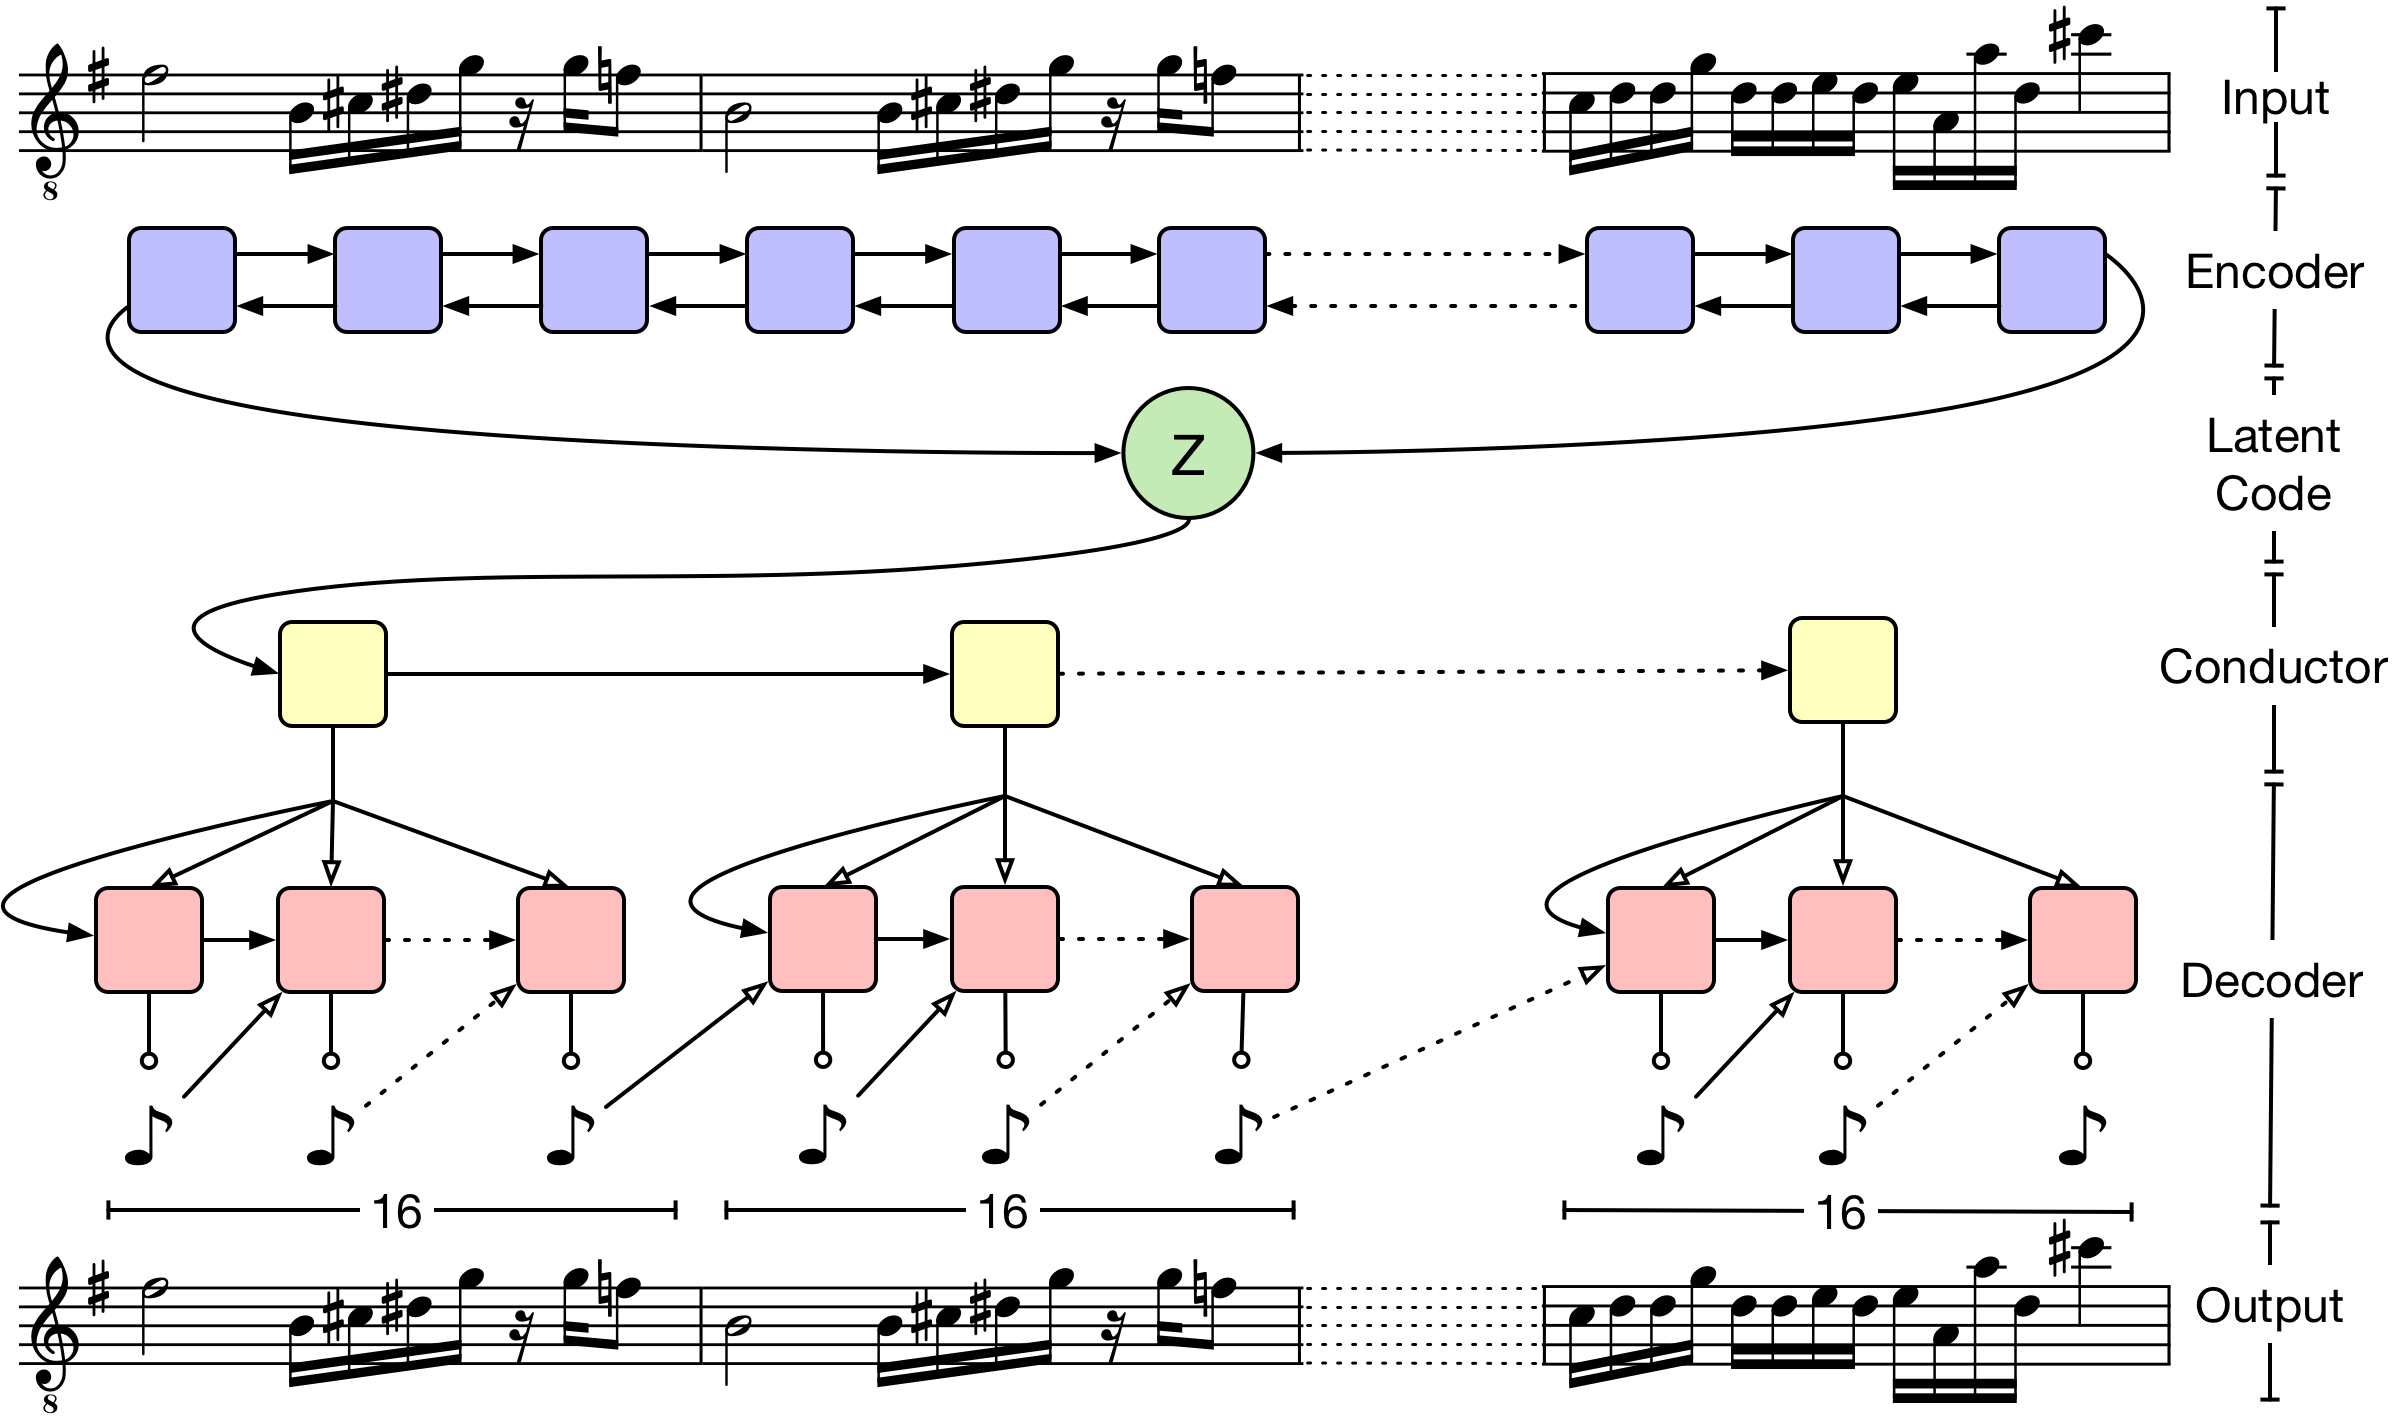
\includegraphics[width=\linewidth]{musicVAE}
\caption{The architecture of the MusicVAE model}
\end{figure}
\end{frame}

\begin{frame}{Résultats}
\begin{itemize}
	\item The hierarchical structure promotes the use of the latent code.
	\item ? Can't generate music out of nothing\dots
	\item \dots but can be used to interpolate between two melody.
	\item \dots
\end{itemize}
\end{frame}

\end{document}
